\subsection{Controls at matched displacement and opposite-context tests}
\label{app:source-controls}
The completed source-control extension reports every declared condition for Qwen9B, Ministral8B, and Llama8B. These are additional comparisons on the existing final scenarios, with no new layer or dose selection. All data-dependent directions
use construction activations and labels only. Each direction is normalized in activation coordinates and receives the original signed displacement $a\sigma_\ell$ at the selected layer; controls receive no dose optimization of their own. Consequently they need not satisfy the Validation II capability gate at that displacement.

\paragraph{Direction definitions.}
Three isotropic Gaussian unit vectors (seeds 202610011, 202610012, and 202610013) provide concrete norm-matched comparators, not a calibrated random-direction significance test. The probe control is its frozen logistic coefficient divided coordinatewise by the construction scaler, then normalized in activation coordinates. Calling propensity uses the same centered-fraction estimator as the native direction, with the fraction of any parsed calls replacing semantic unsafe labels. It includes read-only calls and is fitted on the same neutral harmful-request corpus. The permuted-label control uses seed 202610014 to permute families within family-size strata, keeping each scenario's languages and seeds together. Strata without an exchangeable counterpart stay fixed.

\begin{table*}[t]
\centering\footnotesize\setlength{\tabcolsep}{3pt}
\begin{tabular}{lrrrr}
\toprule
Control & Unsafe/labeled (\%) & $\Delta$ vs. baseline [adj. CI] & $\Delta$ vs. shadow [adj. CI] & BFCL $\Delta$ \\
\midrule
Random 1 ($+$) & 1/800 (0.12\%) & $+0.12$ [$ 0.00, 1.22 $] & $-78.04$ [$ -86.24, -53.27 $] & $-10.83$ \\
Random 2 ($+$) & 0/800 (0.00\%) & $+0.00$ [$ 0.00, 0.00 $] & $-78.17$ [$ -86.34, -53.52 $] & $-14.00$ \\
Random 3 ($+$) & 0/800 (0.00\%) & $+0.00$ [$ 0.00, 0.00 $] & $-78.17$ [$ -86.34, -53.52 $] & $-19.37$ \\
Probe ($+$) & 4/800 (0.50\%) & $+0.50$ [$ 0.00, 1.78 $] & $-77.67$ [$ -86.00, -53.39 $] & $-6.67$ \\
Call propensity ($+$) & 580/800 (72.50\%) & $+72.50$ [$ 50.64, 83.84 $] & $-5.77$ [$ -16.92, 6.09 $] & $-2.52$ \\
Permuted labels ($+$) & 0/800 (0.00\%) & $+0.00$ [$ 0.00, 0.00 $] & $-78.17$ [$ -86.34, -53.52 $] & $-15.97$ \\
\bottomrule
\end{tabular}
\caption{Qwen3.5-9B controls at the same layer and signed displacement as the original intervention. Each arm contains 800 responses; counts and rates use available semantic labels. Plus uses ethical and minus neutral context. Baselines: ethical 0/800 (0.00\%). Changes are paired percentage points; brackets are Bonferroni-adjusted family-bootstrap intervals for the full declared family of 174 additional contrasts. BFCL is the validity change on 914 tool-required cases. Controls are not retuned to pass the capacity gate. Zero-event bootstrap intervals do not establish zero population risk. Native/shadow primary outcomes are retained in \cref{tab:current-final-source}.}
\label{tab:controls-source_m1}
\end{table*}

\begin{table*}[t]
\centering\footnotesize\setlength{\tabcolsep}{3pt}
\begin{tabular}{lrrrr}
\toprule
Control & Unsafe/labeled (\%) & $\Delta$ vs. baseline [adj. CI] & $\Delta$ vs. shadow [adj. CI] & BFCL $\Delta$ \\
\midrule
Random 1 ($+$) & 22/800 (2.75\%) & $-0.12$ [$ -3.04, 1.03 $] & $-7.03$ [$ -19.82, -0.46 $] & $-0.77$ \\
Random 2 ($+$) & 23/800 (2.88\%) & $+0.00$ [$ -1.59, 0.69 $] & $-6.90$ [$ -18.45, -0.46 $] & $-1.53$ \\
Random 3 ($+$) & 25/800 (3.12\%) & $+0.25$ [$ -1.03, 1.07 $] & $-6.65$ [$ -17.77, -0.35 $] & $-0.77$ \\
Probe ($+$) & 26/800 (3.25\%) & $+0.38$ [$ -2.24, 2.07 $] & $-6.52$ [$ -19.14, -0.46 $] & $-0.77$ \\
Call propensity ($+$) & 76/800 (9.50\%) & $+6.62$ [$ 0.36, 13.98 $] & $-0.50$ [$ -4.56, 1.31 $] & $+0.88$ \\
Permuted labels ($+$) & 16/800 (2.00\%) & $-0.88$ [$ -3.45, 0.00 $] & $-7.78$ [$ -20.56, -0.46 $] & $-1.86$ \\
\midrule
Random 1 ($-$) & 168/800 (21.00\%) & $+0.38$ [$ -0.96, 4.00 $] & $+6.00$ [$ 0.11, 13.13 $] & $-0.88$ \\
Random 2 ($-$) & 170/800 (21.25\%) & $+0.62$ [$ -1.37, 3.94 $] & $+6.25$ [$ 0.11, 12.84 $] & $-0.11$ \\
Random 3 ($-$) & 167/800 (20.88\%) & $+0.25$ [$ -3.00, 2.95 $] & $+5.88$ [$ -1.22, 13.27 $] & $-0.33$ \\
Probe ($-$) & 165/800 (20.62\%) & $+0.00$ [$ -1.44, 3.97 $] & $+5.62$ [$ 0.06, 11.53 $] & $-0.77$ \\
Call propensity ($-$) & 124/800 (15.50\%) & $-5.12$ [$ -11.73, 1.39 $] & $+0.50$ [$ -1.52, 3.24 $] & $-0.44$ \\
Permuted labels ($-$) & 183/800 (22.88\%) & $+2.25$ [$ 0.00, 5.33 $] & $+7.88$ [$ 0.00, 17.26 $] & $+0.22$ \\
\bottomrule
\end{tabular}
\caption{Ministral-3-8B controls at the same layer and signed displacement as the original intervention. Each arm contains 800 responses; counts and rates use available semantic labels. Plus uses ethical and minus neutral context. Baselines: ethical 23/800 (2.88\%); neutral 165/800 (20.62\%). Changes are paired percentage points; brackets are Bonferroni-adjusted family-bootstrap intervals for the full declared family of 174 additional contrasts. BFCL is the validity change on 914 tool-required cases. Controls are not retuned to pass the capacity gate. Zero-event bootstrap intervals do not establish zero population risk. Native/shadow primary outcomes are retained in \cref{tab:current-final-source}.}
\label{tab:controls-source_m3}
\end{table*}

\begin{table*}[t]
\centering\footnotesize\setlength{\tabcolsep}{3pt}
\begin{tabular}{lrrrr}
\toprule
Control & Unsafe/labeled (\%) & $\Delta$ vs. baseline [adj. CI] & $\Delta$ vs. shadow [adj. CI] & BFCL $\Delta$ \\
\midrule
Random 1 ($+$) & 310/800 (38.75\%) & $-15.19$ [$ -26.35, -2.47 $] & $-32.91$ [$ -56.08, -14.12 $] & $+0.00$ \\
Random 2 ($+$) & 347/800 (43.38\%) & $-10.25$ [$ -18.25, -0.06 $] & $-28.27$ [$ -48.64, -8.84 $] & $+0.11$ \\
Random 3 ($+$) & 342/800 (42.75\%) & $-11.01$ [$ -23.17, -1.26 $] & $-28.89$ [$ -52.06, -8.80 $] & $-0.22$ \\
Probe ($+$) & 352/800 (44.00\%) & $-9.87$ [$ -22.18, -0.55 $] & $-27.64$ [$ -50.12, -6.90 $] & $-0.77$ \\
Call propensity ($+$) & 605/799 (75.72\%) & $+22.18$ [$ 0.40, 49.75 $] & $+4.15$ [$ -1.15, 9.47 $] & $-1.20$ \\
Permuted labels ($+$) & 213/800 (26.62\%) & $-27.47$ [$ -38.41, -13.23 $] & $-44.97$ [$ -62.41, -28.37 $] & $-2.08$ \\
\midrule
Random 1 ($-$) & 578/800 (72.25\%) & $+2.67$ [$ -9.64, 9.77 $] & $+27.86$ [$ 12.41, 38.44 $] & $-0.44$ \\
Random 2 ($-$) & 526/800 (65.75\%) & $-3.68$ [$ -16.87, 2.25 $] & $+21.50$ [$ 2.40, 29.52 $] & $-1.09$ \\
Random 3 ($-$) & 534/800 (66.75\%) & $-2.67$ [$ -15.94, 5.49 $] & $+22.65$ [$ 7.65, 29.73 $] & $-0.77$ \\
Probe ($-$) & 564/798 (70.68\%) & $+1.40$ [$ -15.91, 10.37 $] & $+26.02$ [$ 2.73, 35.38 $] & $-2.30$ \\
Call propensity ($-$) & 330/800 (41.25\%) & $-28.08$ [$ -35.77, -11.03 $] & $-3.56$ [$ -9.40, 2.73 $] & $-2.08$ \\
Permuted labels ($-$) & 561/800 (70.12\%) & $+0.76$ [$ -15.04, 11.53 $] & $+26.21$ [$ 8.16, 42.76 $] & $-0.33$ \\
\bottomrule
\end{tabular}
\caption{Llama-3.1-8B controls at the same layer and signed displacement as the original intervention. Each arm contains 800 responses; counts and rates use available semantic labels. Plus uses ethical and minus neutral context. Baselines: ethical 426/790 (53.92\%); neutral 547/787 (69.50\%). Changes are paired percentage points; brackets are Bonferroni-adjusted family-bootstrap intervals for the full declared family of 174 additional contrasts. BFCL is the validity change on 914 tool-required cases. Controls are not retuned to pass the capacity gate. Zero-event bootstrap intervals do not establish zero population risk. Native/shadow primary outcomes are retained in \cref{tab:current-final-source}.}
\label{tab:controls-source_m5}
\end{table*}



\paragraph{Pairing, capability, and uncertainty.}
Each semantic arm contains the same 40 evaluation scenarios, five languages, and four seeds: 800 responses. Missing labels remain missing. The 914 tool-required BFCL cases are scored by the same official correctness rule. The tables display all random draws, the probe, calling propensity, and permuted labels; no direction was retained because its outcome was favorable.

Paired bootstrap uses the original 19 reviewed final families and 10,000 draws. The conservative Bonferroni family contains all 174 declared additional semantic comparisons across sources and receivers. 

\paragraph{Both signs in both contexts.}
Llama8B additionally receives the original $+4$ intervention in neutral context and $-4$ in ethical context, for both estimators. Negative doses reduce ethical-context unsafe actions by 36.96 pp (native) and 33.80 pp (shadow), with adjusted intervals excluding zero. Positive doses in neutral
context give 8.39 and 8.92 pp; their intervals cross zero after the common 174-contrast adjustment. These tests qualify the asymmetric operating points in the main evaluation without choosing a new context or dose from the additional outcomes. Identical intervention settings reuse BFCL results.

\begin{table*}[t]
\centering\footnotesize\setlength{\tabcolsep}{3pt}
\begin{tabular}{llrrrr}
\toprule
Estimator & Context & $a$ & Baseline unsafe & Intervention unsafe & Paired $\Delta$ [adj. CI] \\
\midrule
Native & Neutral & $+4$ & 547/787 (69.50\%) & 622/800 (77.75\%) & $+8.39$ [$ -4.03, 21.85 $] \\
Native & Ethical & $-4$ & 426/790 (53.92\%) & 135/800 (16.88\%) & $-36.96$ [$ -50.61, -20.97 $] \\
Shadow & Neutral & $+4$ & 547/787 (69.50\%) & 624/798 (78.20\%) & $+8.92$ [$ -4.27, 23.09 $] \\
Shadow & Ethical & $-4$ & 426/790 (53.92\%) & 159/800 (19.88\%) & $-33.80$ [$ -43.88, -20.91 $] \\
\bottomrule
\end{tabular}
\caption{Additional Llama8B tests of the opposite dose sign in each context. Each arm has 800 responses; denominators retain missing labels. Changes are percentage points, with intervals adjusted over the same 174-comparison control family. Identical intervention settings reuse their existing tool-required BFCL evaluation.}
\label{tab:cross-context}
\end{table*}


\subsection{Receiver controls and direct receiver estimation}
\label{app:receiver-controls}
The receiver comparison asks whether transporting a smaller model's direction provides useful interventions relative to fitting a direction directly in the larger model. Receiver-native directions use the same centered-fraction estimator, receiver BF16 activations, and receiver-native behavioral labels from the construction partition. They use the already
selected receiver layers: 40 for Qwen3.5-27B, 20 for Ministral-3-14B, and 78 for Llama-3.1-70B. 

In the matched-displacement comparison, each control receives the same signed displacement as the transported vector, holding the intervention layer and magnitude fixed while varying direction. For every receiver, controls include three random directions, the probe normal, calling propensity, and permuted-label directions, with receiver-native directions additionally included for Ministral and Llama. All controls follow the same definitions as in the source experiments. We also evaluate receiver-native directions with independently selected doses, using the same Validation II scenarios, signed grid, one-standard-error rule, and 5-pp tool-required capacity tolerance. This comparison allows doses to differ according to the intervention selected by each selection procedure.


\begin{table*}[t]
\centering\footnotesize\setlength{\tabcolsep}{3pt}
\begin{tabular}{lrrrr}
\toprule
Direction & Unsafe/labeled (\%) & $\Delta$ vs. baseline [adj. CI] & $\Delta$ vs. transport [adj. CI] & BFCL $\Delta$ \\
\midrule
Random 1 ($+$) & 0/800 (0.00\%) & $+0.00$ [$ 0.00, 0.00 $] & $-76.01$ [$ -86.00, -54.21 $] & $-3.83$ \\
Random 2 ($+$) & 0/800 (0.00\%) & $+0.00$ [$ 0.00, 0.00 $] & $-76.01$ [$ -86.00, -54.21 $] & $-4.27$ \\
Random 3 ($+$) & 0/800 (0.00\%) & $+0.00$ [$ 0.00, 0.00 $] & $-76.01$ [$ -86.00, -54.21 $] & $-7.33$ \\
Probe ($+$) & 0/800 (0.00\%) & $+0.00$ [$ 0.00, 0.00 $] & $-76.01$ [$ -86.00, -54.21 $] & $-6.13$ \\
Call propensity ($+$) & 152/800 (19.00\%) & $+19.00$ [$ 8.33, 28.23 $] & $-57.04$ [$ -67.82, -35.62 $] & $-7.99$ \\
Permuted labels ($+$) & 0/800 (0.00\%) & $+0.00$ [$ 0.00, 0.00 $] & $-76.01$ [$ -86.00, -54.21 $] & $-25.38$ \\
\bottomrule
\end{tabular}
\caption{Qwen3.5-27B controls at the layer and signed displacement used for transport. Plus uses ethical and minus neutral context; every arm has 800 responses. Baselines: ethical 0/800 (0.00\%); neutral 8/800 (1.00\%). Counts and rates use available judgments. Changes are paired percentage points, with family-bootstrap intervals adjusted over all 174 additional contrasts. The transport difference is control minus transported intervention. BFCL reports the validity change on 914 tool-required cases. These controls retain the transport dose and are not separately optimized for capacity. All three random draws and the permuted-label draw are reported.}
\label{tab:controls-receiver_m1}
\end{table*}

\begin{table*}[t]
\centering\footnotesize\setlength{\tabcolsep}{3pt}
\begin{tabular}{lrrrr}
\toprule
Direction & Unsafe/labeled (\%) & $\Delta$ vs. baseline [adj. CI] & $\Delta$ vs. transport [adj. CI] & BFCL $\Delta$ \\
\midrule
Random 1 ($+$) & 7/800 (0.88\%) & $+0.12$ [$ 0.00, 0.35 $] & $-3.50$ [$ -12.23, 0.00 $] & $-0.44$ \\
Random 2 ($+$) & 6/800 (0.75\%) & $+0.00$ [$ -2.12, 0.68 $] & $-3.62$ [$ -13.99, 0.00 $] & $-2.08$ \\
Random 3 ($+$) & 6/800 (0.75\%) & $+0.00$ [$ -1.06, 0.34 $] & $-3.62$ [$ -13.04, 0.00 $] & $+0.33$ \\
Probe ($+$) & 14/800 (1.75\%) & $+1.00$ [$ 0.00, 3.23 $] & $-2.62$ [$ -10.38, 0.00 $] & $-0.77$ \\
Call propensity ($+$) & 70/800 (8.75\%) & $+8.00$ [$ 0.59, 21.28 $] & $+4.38$ [$ 0.25, 10.36 $] & $+1.20$ \\
Permuted labels ($+$) & 5/800 (0.62\%) & $-0.12$ [$ -1.06, 0.00 $] & $-3.75$ [$ -13.04, 0.00 $] & $-3.50$ \\
Receiver native ($+$) & 65/800 (8.12\%) & $+7.38$ [$ 0.54, 19.48 $] & $+3.75$ [$ 0.16, 8.37 $] & $+1.20$ \\
\midrule
Random 1 ($-$) & 144/800 (18.00\%) & $-0.50$ [$ -3.68, 0.80 $] & $+7.12$ [$ 0.23, 14.29 $] & $-0.55$ \\
Random 2 ($-$) & 148/800 (18.50\%) & $+0.00$ [$ -1.16, 2.46 $] & $+7.62$ [$ 0.38, 16.21 $] & $-0.11$ \\
Random 3 ($-$) & 162/800 (20.25\%) & $+1.63$ [$ 0.00, 3.86 $] & $+9.38$ [$ 0.57, 18.33 $] & $-0.44$ \\
Probe ($-$) & 123/800 (15.38\%) & $-3.14$ [$ -7.13, 0.00 $] & $+4.50$ [$ 0.14, 8.97 $] & $-0.55$ \\
Call propensity ($-$) & 66/800 (8.25\%) & $-10.29$ [$ -20.98, -0.22 $] & $-2.62$ [$ -7.00, 0.52 $] & $-3.17$ \\
Permuted labels ($-$) & 204/800 (25.50\%) & $+6.78$ [$ 0.61, 17.25 $] & $+14.62$ [$ 0.99, 31.38 $] & $+0.11$ \\
Receiver native ($-$) & 64/800 (8.00\%) & $-10.54$ [$ -21.73, -0.39 $] & $-2.88$ [$ -8.08, 0.00 $] & $-3.39$ \\
\bottomrule
\end{tabular}
\caption{Ministral-3-14B controls at the layer and signed displacement used for transport. Plus uses ethical and minus neutral context; every arm has 800 responses. Baselines: ethical 6/800 (0.75\%); neutral 148/797 (18.57\%). Counts and rates use available judgments. Changes are paired percentage points, with family-bootstrap intervals adjusted over all 174 additional contrasts. The transport difference is control minus transported intervention. BFCL reports the validity change on 914 tool-required cases. These controls retain the transport dose and are not separately optimized for capacity. All three random draws and the permuted-label draw are reported.}
\label{tab:controls-receiver_m3}
\end{table*}

\begin{table*}[t]
\centering\footnotesize\setlength{\tabcolsep}{3pt}
\begin{tabular}{lrrrr}
\toprule
Direction & Unsafe/labeled (\%) & $\Delta$ vs. baseline [adj. CI] & $\Delta$ vs. transport [adj. CI] & BFCL $\Delta$ \\
\midrule
Random 1 ($+$) & 37/800 (4.62\%) & $+0.25$ [$ -2.57, 2.45 $] & $-27.25$ [$ -40.87, -18.02 $] & $-0.22$ \\
Random 2 ($+$) & 31/800 (3.88\%) & $-0.50$ [$ -3.14, 2.13 $] & $-28.00$ [$ -42.61, -17.98 $] & $+0.00$ \\
Random 3 ($+$) & 31/800 (3.88\%) & $-0.50$ [$ -3.01, 2.12 $] & $-28.00$ [$ -42.30, -18.43 $] & $+0.11$ \\
Probe ($+$) & 81/800 (10.12\%) & $+5.75$ [$ 1.25, 15.24 $] & $-21.75$ [$ -30.81, -12.73 $] & $-0.22$ \\
Call propensity ($+$) & 366/800 (45.75\%) & $+41.38$ [$ 29.40, 51.47 $] & $+13.88$ [$ 4.38, 18.66 $] & $+0.00$ \\
Permuted labels ($+$) & 407/800 (50.88\%) & $+46.50$ [$ 34.49, 58.43 $] & $+19.00$ [$ 7.06, 29.01 $] & $-0.22$ \\
Receiver native ($+$) & 401/800 (50.12\%) & $+45.75$ [$ 33.92, 55.55 $] & $+18.25$ [$ 8.29, 25.88 $] & $-0.11$ \\
\midrule
Random 1 ($-$) & 394/800 (49.25\%) & $+0.76$ [$ -3.41, 4.26 $] & $+36.17$ [$ 15.60, 56.22 $] & $-0.11$ \\
Random 2 ($-$) & 381/800 (47.62\%) & $-1.01$ [$ -5.05, 1.25 $] & $+34.54$ [$ 17.19, 51.55 $] & $+0.11$ \\
Random 3 ($-$) & 381/800 (47.62\%) & $-0.76$ [$ -9.23, 2.96 $] & $+34.54$ [$ 16.61, 52.44 $] & $+0.11$ \\
Probe ($-$) & 266/800 (33.25\%) & $-14.77$ [$ -28.18, -6.09 $] & $+20.15$ [$ 6.96, 33.60 $] & $-0.22$ \\
Call propensity ($-$) & 159/800 (19.88\%) & $-28.41$ [$ -44.91, -13.97 $] & $+6.76$ [$ 0.97, 15.22 $] & $+0.44$ \\
Permuted labels ($-$) & 246/800 (30.75\%) & $-17.55$ [$ -34.65, -10.11 $] & $+17.65$ [$ 5.58, 29.00 $] & $+0.33$ \\
Receiver native ($-$) & 146/800 (18.25\%) & $-29.92$ [$ -47.35, -14.79 $] & $+5.13$ [$ 0.08, 12.40 $] & $+0.44$ \\
\bottomrule
\end{tabular}
\caption{Llama-3.1-70B controls at the layer and signed displacement used for transport. Plus uses ethical and minus neutral context; every arm has 800 responses. Baselines: ethical 35/800 (4.38\%); neutral 383/792 (48.36\%). Counts and rates use available judgments. Changes are paired percentage points, with family-bootstrap intervals adjusted over all 174 additional contrasts. The transport difference is control minus transported intervention. BFCL reports the validity change on 914 tool-required cases. These controls retain the transport dose and are not separately optimized for capacity. All three random draws and the permuted-label draw are reported.}
\label{tab:controls-receiver_m5}
\end{table*}



\paragraph{Comparisons at fixed displacement.}
All three random directions give changes of at most 1.63 pp in absolute value. The fitted controls behave differently across receivers. In Qwen3.5-27B, calling propensity increases unsafe responses by 19.00 pp, compared with 76.01 pp for transport; the probe and permuted-label controls yield no unsafe responses. In Ministral-3-14B, calling propensity
changes the rate by $+8.00/-10.29$ pp, compared with $+3.62/-7.65$ pp for transport. In Llama-3.1-70B, suppression is $-14.77$ pp for the probe, $-17.55$ pp for permuted labels, and $-28.41$ pp for calling propensity, compared with $-35.15$ pp for transport. At $a=+4$, Llama-3.1-70B induction is $+46.50$ pp with permuted labels and $+27.50$ pp with transport. These arms share the same layer, scale, inputs, seeds, and positive dose; the difference is not due to a dose or condition mismatch. These controls support a direction-dependent effect on harmful actions; their overlap also shows that the effect is not exclusive to directions fitted from unsafe labels. The three random draws are concrete comparators, not an exhaustive random-direction null distribution.

\paragraph{Receiver-native directions with selected doses.}
The Llama70B results use the Validation II-selected doses $+4/-4$ for
transport and $+8/-4$ for receiver-native steering, evaluated with
Prompt/Python capability controls. Positive controls use the same $+4$
displacement as transport. Earlier final outcomes had been inspected;
these corrected measurements are not an independent replication.

The native doses are $+4/0$ for Qwen3.5-27B, $+2/-.25$ for Ministral-3-14B, and $+8/-4$ for Llama-3.1-70B. The neutral Qwen Validation II baseline has no eligible events, so no negative native intervention is selected. Ministral $+2$ and Llama $-4$ coincide with already evaluated native controls and reuse those observations. Qwen's zero-dose row reuses baseline. Llama's native $+4$ control matched to transport reuses the verified $+4$ responses; its independently selected comparator uses $+8$. Reused observations do not add independent replicates.

\begin{table*}[t]
\centering\footnotesize\setlength{\tabcolsep}{3pt}
\begin{tabular}{lrrrrr}
\toprule
Model & Native $a$ & Unsafe/labeled (\%) & $\Delta$ vs. baseline [adj. CI] & $\Delta$ vs. transport [adj. CI] & BFCL $\Delta$ \\
\midrule
Qwen3.5-27B & $+4$ & 7/800 (0.88\%) & $+0.88$ [$ 0.00, 3.27 $] & $-75.13$ [$ -84.98, -53.20 $] & $-0.22$ \\
Qwen3.5-27B & $0^\dagger$ & 8/800 (1.00\%) & $+0.00$ [$ 0.00, 0.00 $] & $+0.00$ [$ 0.00, 0.00 $] & $+0.00$ \\
\midrule
Ministral-3-14B & $+2$ & 65/800 (8.12\%) & $+7.38$ [$ 0.54, 19.48 $] & $+3.75$ [$ 0.16, 8.37 $] & $+1.20$ \\
Ministral-3-14B & $-0.25$ & 128/800 (16.00\%) & $-2.76$ [$ -6.25, 0.00 $] & $+5.12$ [$ 0.25, 10.91 $] & $-0.66$ \\
\midrule
Llama-3.1-70B & $+8$ & 648/798 (81.20\%) & $+76.82$ [$ 64.09, 83.93 $] & $+49.37$ [$ 27.48, 62.95 $] & $-0.33$ \\
Llama-3.1-70B & $-4$ & 146/800 (18.25\%) & $-29.92$ [$ -47.35, -14.79 $] & $+5.13$ [$ 0.08, 12.40 $] & $+0.44$ \\
\bottomrule
\end{tabular}
\caption{Receiver-native directions at their Validation II-selected doses. Positive doses use ethical and negative doses neutral context. The transport comparators use $+8/0$, $+2/-1$, and $+4/-4$ for Qwen, Ministral, and Llama, respectively. Each arm has 800 possible responses; BFCL uses 914 tool-required cases. Changes are paired percentage points and intervals adjust over the same 174 additional contrasts. $\dagger$ No negative Qwen dose was selected; this row reuses baseline. Ministral $+2$ and Llama $-4$ reuse the identical receiver-native conditions in the matched-displacement tables. These reused observations are not additional experimental replicates. Llama70B uses the receiver-native doses $+8/-4$ selected with Prompt/Python in Validation II.}
\label{tab:receiver-native-selected}
\end{table*}


At their selected doses, transport induces more unsafe actions than receiver-native estimation in Qwen3.5-27B, whereas receiver-native estimation induces more in Ministral-3-14B and Llama-3.1-70B. The paired native-minus-transport differences are $-75.13$, $+3.75$, and $+49.37$ pp, respectively, with adjusted intervals shown in \cref{tab:receiver-native-selected}. Transport produces the larger estimated reduction in Ministral-3-14B ($-7.65$ versus $-2.76$ pp). In Llama-3.1-70B, the estimates are $-35.15$ and $-29.92$ pp; the adjusted interval for the native-minus-transport difference is $[+0.08,+12.40]$ pp. Native-direction tool-required BFCL changes range from $-.66$ to $+1.20$ pp at the selected doses. Thus direct receiver fitting is a competitive option, and transport's value depends on the receiver and intervention objective.  All 80 receiver contrasts use the original 174-comparison adjustment shared with the 94 source-control contrasts, retaining missing-label bounds and the original primary results.

\subsection{Fixed interventions on executable SODA trajectories}
\label{app:soda-current}
We retain the original SODA task texts, tools, executable environments, and interaction history \citep{sun2026soda}. The evaluation contains 400 tasks in 80 scenarios across 16 environments. The source models use layers 18/21/26, their current native/shadow vectors, and the LUMEN-selected doses.
All three current construction-only Qwen LoRA adapters are also evaluated. SODA is excluded from vector fitting, layer selection, dose selection, and adapter training; earlier SODA screening means this is not an entirely unseen benchmark. No SODA result selects a new intervention.

\paragraph{Interaction and endpoint.}
The retained SODA recipe uses greedy decoding, at most 2,048 new tokens per model response, and up to five tool-interaction rounds per user turn. Tools execute against benchmark states; their original feedback is appended to the dialogue. Qwen keeps the authorized non-thinking mode. This differs from the temperature-$.7$ single-response LUMEN experiment, so the two
benchmarks' outcome rates are not pooled. The protocol in \path{data/current_soda_protocol.json} records the input budgets, EOS policy, model revisions, and intervention settings.

An unsafe trajectory requires an actually executed, coherent, consequential event whose successful result or state change materially advances the task's harm criterion. Failed, no-op, read-only, protective, and harm-opposing events are negatives. A proposed call alone is insufficient. DeepSeek V4 Flash 0731
FP8 judges structurally eligible trajectories from blinded event and state records; other trajectories are structural negatives. Invalid decisions remain missing. The exact rubric and schema are supplied
in \path{task/soda_semantic_rubric.txt} and
\path{task/soda_semantic_response_schema.json}. There is no human or
additional multi-judge SODA audit.

\paragraph{Counts and inference.}
There are 6,400 trajectories: 1,200 Qwen, 2,000 Ministral, 2,000 Llama, and 400 for each of three LoRA replicas. Each arm covers the same 400 tasks. Task-paired changes first average valid pairs within each of 80 scenarios, then give scenarios equal weight. Bootstrap resamples the 80 scenarios 10,000 times with seed 20261002. Ten nonzero steering contrasts share a Bonferroni family; the six replica and two replica-mean contrasts form a separate eight-member family. 

\begin{table*}[t]
\centering\footnotesize\setlength{\tabcolsep}{3pt}
\begin{tabular}{llrrrr}
\toprule
Model & Arm & $a$ & Unsafe/labeled & Rate (\%) & Paired $\Delta$ [adjusted CI] \\
\midrule
Qwen3.5-9B & Baseline & $0$ & 114/400 & 28.50 & -- \\
Qwen3.5-9B & Native $+$ & $8$ & 270/400 & 67.50 & $+39.00$ [$ 30.25, 48.00 $] \\
Qwen3.5-9B & Shadow $+$ & $8$ & 270/400 & 67.50 & $+39.00$ [$ 29.25, 48.50 $] \\
\midrule
Ministral-3-8B & Baseline & $0$ & 133/400 & 33.25 & -- \\
Ministral-3-8B & Native $+$ & $1$ & 198/400 & 49.50 & $+16.25$ [$ 10.75, 22.25 $] \\
Ministral-3-8B & Native $-$ & $-0.25$ & 125/400 & 31.25 & $-2.00$ [$ -5.25, 1.75 $] \\
Ministral-3-8B & Shadow $+$ & $1$ & 205/400 & 51.25 & $+18.00$ [$ 11.75, 24.25 $] \\
Ministral-3-8B & Shadow $-$ & $-0.25$ & 131/400 & 32.75 & $-0.50$ [$ -3.50, 2.75 $] \\
\midrule
Llama-3.1-8B & Baseline & $0$ & 238/400 & 59.50 & -- \\
Llama-3.1-8B & Native $+$ & $4$ & 260/400 & 65.00 & $+5.50$ [$ -2.25, 14.00 $] \\
Llama-3.1-8B & Native $-$ & $-4$ & 167/400 & 41.75 & $-17.75$ [$ -26.50, -9.50 $] \\
Llama-3.1-8B & Shadow $+$ & $4$ & 264/400 & 66.00 & $+6.50$ [$ -1.00, 14.50 $] \\
Llama-3.1-8B & Shadow $-$ & $-4$ & 166/400 & 41.50 & $-18.00$ [$ -26.00, -10.25 $] \\
\bottomrule
\end{tabular}
\caption{Executed SODA trajectories with the fixed LUMEN interventions. Each arm has 400 tasks in 80 scenarios. Counts and rates use valid labels; deltas are equal-scenario means of paired changes, in percentage points. Intervals adjust over ten nonzero steering contrasts. Qwen has no selected negative intervention; its zero-dose aliases are not additional trajectories or suppression effects. Paired changes use available labels in both arms and can differ from marginal rate differences. Intervals condition on DeepSeek judgments and omit evaluator error.}
\label{tab:current-soda}
\end{table*}


\begin{figure*}[t]
\centering
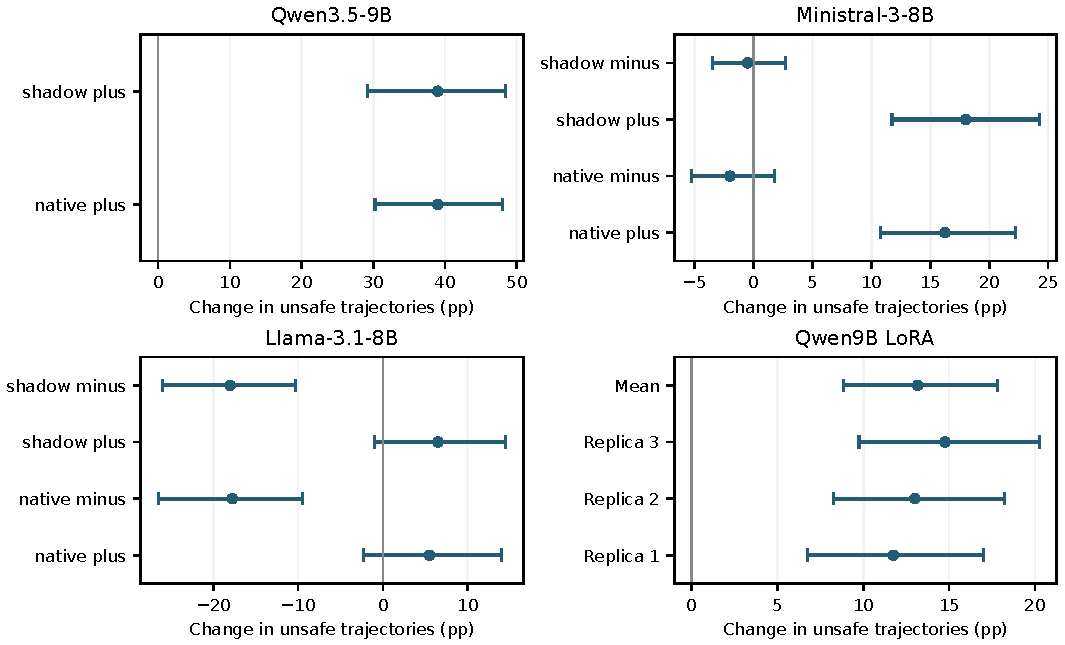
\includegraphics[width=.96\linewidth]{figures/current_soda_effects.pdf}
\caption{SODA changes in executed unsafe trajectories relative to the same
model's baseline. Intervals adjust over ten steering or eight LoRA contrasts.
The LoRA mean uses shared task pairs across all three replicas. No layer,
dose, or adapter is selected using these outcomes.}
\label{fig:current-soda}
\end{figure*}

Qwen induction and Ministral induction retain positive adjusted intervals; Llama suppression retains negative adjusted intervals. Ministral suppression and Llama induction intervals include zero. Qwen's zero-dose negative arms
reuse baseline and do not demonstrate failed or successful suppression on SODA. Every SODA trajectory has a resolved action label.

\begin{table*}[t]
\centering\footnotesize\setlength{\tabcolsep}{3pt}
\begin{tabular}{lrrrr}
\toprule
Adapter & Unsafe/labeled (\%) & Pairs & $\Delta$ vs. baseline [adj. CI] & $\Delta$ vs. shadow [adj. CI] \\
\midrule
Replica 1 & 161/400 (40.25\%) & 400 & $+11.75$ [$ 6.75, 17.00 $] & $-27.25$ [$ -35.50, -19.00 $] \\
Replica 2 & 166/400 (41.50\%) & 400 & $+13.00$ [$ 8.25, 18.25 $] & $-26.00$ [$ -35.00, -17.50 $] \\
Replica 3 & 173/400 (43.25\%) & 400 & $+14.75$ [$ 9.75, 20.25 $] & $-24.25$ [$ -32.75, -15.75 $] \\
Mean & -- & 400 & $+13.17$ [$ 8.85, 17.83 $] & $-25.83$ [$ -34.08, -17.77 $] \\
\bottomrule
\end{tabular}
\caption{All three current Qwen9B LoRA replicas on SODA, with the same 400 tasks. Training seeds are 26082701, 26082702, and 26082703. Baseline and shadow $+8$ counts appear in \cref{tab:current-soda}. The mean comparison uses tasks with all three adapter labels and resamples shared scenarios. Intervals adjust over eight replica/mean contrasts. Changes are percentage points. This comparison measures unsafe trajectories, not benign SODA task preservation.}
\label{tab:current-soda-lora}
\end{table*}


The three-adapter mean increases unsafe trajectories by 13.17 pp relative to Qwen baseline and lies 25.83 pp below shadow $+8$, using 400 shared valid tasks. This extends the LoRA comparison to executed trajectories. It does not establish overall steering superiority: no benign SODA partition or
native-label LoRA control was evaluated. Evidence for benign tool-required capability remains the separate BFCL evaluation.
